\documentclass[a4paper,12pt]{article}

% Définition des packages et de leurs paramètres

\usepackage{graphicx}  % Pour insérer des images
\usepackage{textpos}   % Pour positionner précisément les images
\usepackage[french]{babel}  % Utiliser le package babel pour le français
\usepackage{csquotes}         % Ajouter csquotes pour babel
\usepackage[T1]{fontenc}      % Corriger l'encodage pour le français
\usepackage[colorlinks=true, linkcolor=blue]{hyperref}  % Liens cliquables en bleu sans les encadrer
\usepackage{amssymb}    % pour les symboles mathématiques
\usepackage{float}      % Pour le placement précis des figures avec [H]
\usepackage{microtype}

\usepackage{geometry}  % Pour ajuster les marges
\geometry{top=2cm, bottom=2cm, left=2cm, right=2cm}

% Ajout d'un espace insécable entre les décimales
\usepackage{siunitx}
\sisetup{output-decimal-marker = {,}, group-separator = {\,}, group-minimum-digits = 4}


\usepackage[style=apa, backend=biber]{biblatex}
\addbibresource{references.bib}

\usepackage{tocloft} % Pour modifier l'apparence du sommaire
\setlength{\cftbeforesecskip}{10pt} % Espacement entre les sections
\setlength{\cftbeforesubsecskip}{8pt} % Espacement entre les sous-sections
\renewcommand{\cftsecleader}{\cftdotfill{\cftdotsep}}
\setlength{\cftaftertoctitleskip}{25pt} % Espace sous le titre du sommaire

% Informations du document

\title{Projet Pl@ntnet}
\author{Émilie Aigoin}
\date{January 2025}

\begin{document}

% Logo de l'université en haut à gauche
\begin{textblock*}{3cm}(0.01cm,0.2cm)
    
\includegraphics[width=4cm]{images/Universite.png}
\end{textblock*}

% Logo du master en haut à droite
\begin{textblock*}{3cm}(11cm,1cm)
    
\includegraphics[width=6cm]{images/SSD.png} 
\end{textblock*}

% Titre principal
\vspace{8cm}
\begin{center}
\large{Projet de master présenté dans le contexte de l'UE HAX817X} \\ \vspace{0.4cm}
    {\LARGE \textbf{Prédiction conformelle et base de données \\ \vspace{0.4cm} Pl@ntNet-CrowdSWE}}\\[1cm]
\end{center}

% Logo de l'application centré
\begin{textblock*}{3cm}(5cm,0.5cm)
    
\includegraphics[width=6cm]{images/plantenet.png}  % Remplacer par le bon fichier
\end{textblock*}

% Informations
\vfill
\begin{center}
Présenté par \\ \vspace{0.2cm}
    {\textbf{AIGOIN Emilie \\ \vspace{0.1cm} CLETZ Laura \\ \vspace{0.1cm} THOMAS Anne-Laure}}\\ \vspace{0.6cm}
    
Sous la direction (ou co-direction) de \\ \vspace{0.2cm}
    {\textbf{BOTELLA Christophe \\ \vspace{0.1cm} SALMON Joseph }}\\ \vspace{1.5cm}
    
    {\large Master Statistique et Science des Données, \\ \vspace{0.1cm} Université de Montpellier}\\ \vspace{0.6cm}
    {\large Année 2024 - 2025}
\end{center}

% Page de garde sans numéro de page
\thispagestyle{empty}

\newpage

% Insertion du sommaire
\tableofcontents 

\newpage

%%%%%%%%%%%%%%%%%%%%%%%%%%%%%%%%%%%%%%%%%%%%%%%%%%%%%%%%%%%%%%%%%%%%%%%%%%%%%%%%
%%%%%%%%%%%%%%%%%%%%%%%%%%%%%%%%%%%%%%%%%%%%%%%%%%%%%%%%%%%%%%%%%%%%%%%%%%%%%%%%

\section{Introduction}

La reconnaissance des plantes est une problématique clé en botanique, avec des applications directes dans la conservation de la biodiversité, la gestion des écosystèmes ou encore la culture personnelle. Parmi les initiatives les plus importantes dans ce domaine, le projet Pl@ntNet joue un rôle central en proposant une application de reconnaissance automatique des plantes basée sur des données collectées par les utilisateurs. Cette approche de science participative permet de constituer une base de données massive et diversifiée de plus de $6$ millions d'observations pour la seule région de l'Europe du Sud-Ouest, impliquant plus de $\num{800000}$ contributeurs et couvrant plus de $\num{17000}$ espèces végétales. Ce qui est essentiel pour entraîner et affiner les modèles de classification.

\vspace{0.2cm}

Cependant, garantir la fiabilité des prédictions reste un défi majeur. Les données collectées, bien que nombreuses, peuvent être de qualité variable en raison des conditions de prise de vue (lumière, angle, netteté), de la diversité des espèces et de l'expertise variable des contributeurs. Pour améliorer la précision de l'application, il ne suffit pas d’optimiser la classification : nous devons également quantifier l’incertitude des prédictions et adapter dynamiquement la sortie du modèle en fonction du niveau de confiance.

\vspace{0.2cm}

Dans ce travail, nous nous sommes intégrées au projet Pl@ntNet avec un objectif précis : améliorer la fiabilité des prédictions en les rendant adaptatives. Plutôt que de fournir une unique réponse avec une probabilité associée, notre objectif était de générer un ensemble de prédictions dont la probabilité de contenir la bonne espèce atteint un niveau de garantie satisfaisant (fixé comme étant $95\%$). Cet ensemble doit être le plus restreint possible pour éviter les suggestions inutiles, tout en s'ajustant automatiquement en fonction de la difficulté de l’identification : être plus précis pour les cas évidents et plus large pour les situations ambiguës.

\vspace{0.2cm}

Pour répondre à cette problématique, nous avons utilisé la prédiction conforme, une approche statistique permettant de transformer les sorties probabilistes d'un modèle de classification en ensembles de prédiction avec des garanties de couverture. Contrairement aux méthodes classiques, la prédiction conforme offre des garanties valides même pour des échantillons de taille finie et sans hypothèses fortes sur la distribution des données.

\vspace{0.2cm}

Dans la suite de ce rapport, nous détaillerons notre approche en commençant par une présentation approfondie de l'application Pl@ntnet et des données utilisées, suivie d'analyses statistiques descriptives. Nous introduirons ensuite le cadre théorique de la prédiction conforme avant de présenter notre méthodologie, nos résultats principaux et leurs implications pour l'amélioration de l'application.

%%%%%%%%%%%%%%%%%%%%%%%%%%%%%%%%%%%%%%%%%%%%%%%%%%%%%%%%%%%%%%%%%%%%%%%%%%%%%%%%
%%%%%%%%%%%%%%%%%%%%%%%%%%%%%%%%%%%%%%%%%%%%%%%%%%%%%%%%%%%%%%%%%%%%%%%%%%%%%%%%

\section{Jeux de données et outils}

%%%%%%%%%%%%%%%%%%%%%%%%%%%%%%%%%%%%%%%%%%%%%%%%%%%%%%%%%%%%%%%%%%%%%%%%%%%%%%%%

\subsection{Application Pl@ntnet}

Pl@ntNet est un projet de sciences participatives accessible sous forme d’application mobile gratuite, mais également via une \href{https://identify.plantnet.org/fr}{interface en ligne}. Développé conjointement par l'Institut National de Recherche Informatique et Automatique (INRIA), le Centre de coopération International en Recherche Agronomique (CIRAD) et l'Institut de Recherche pour le Développement (IRD), ce projet a été lancé en $2009$ et recense plus de $20$ millions d'utilisateurs dans le monde en $2024$. 

\vspace{0.2cm}

Son objectif principal est d'aider le grand public et les professionnels à identifier les espèces végétales à partir de photographies. L'application s'appuie sur des algorithmes d'intelligence artificielle qui analysent les caractéristiques visuelles des plantes (écorce, feuilles, fruits, fleurs, etc.) pour proposer des identifications. Au-delà de la reconnaissance des plantes, Pl@ntnet permet également de cartographier la distribution géographique des espèces végétales en fonction de la localisation des photographies partagées par les utilisateurs.

\vspace{0.2cm}

Pl@ntNet est basée sur un principe d’apprentissage coopératif et itératif. Les utilisateurs peuvent partager leurs photographies (que nous appellerons des observations) et celles-ci peuvent être ensuite révisées par la communauté. Cet autre type de contribution est utilisé non seulement pour enrichir la base de données, mais est aussi utilisé par l’IA pour améliorer les performances de son système de reconnaissance. Les utilisateurs peuvent, par exemple, confirmer l'identification d'une espèce, suggérer une identification alternative ou signaler une erreur.

\vspace{0.2cm}

Le processus fonctionne ainsi : lorsqu'un utilisateur soumet une photographie, l'algorithme d'intelligence artificielle analyse l'image et génère une liste d'espèces candidates (appelées étiquettes), chacune associée à une probabilité. L'espèce affichée en première position est celle que l'intelligence artificielle estime la plus probable, suivie des autres classées par ordre décroissant de probabilité. Pour garantir la pertinence des suggestions et ne pas surcharger l'utilisateur d'informations avec des espèces peu probables, l'affichage est limité aux espèces dont la probabilité dépasse le seuil minimal, fixé à $0,001$ (soit $0,1\%$).

\vspace{0.2cm}

Notre travail est basé sur une démarche d'optimisation de ce système, avec pour objectif de rendre le nombre d'étiquettes présentées adaptatif à la difficulté du problème d'identification : plus l'identification est facile, moins le système proposera d'options à l'utilisateur, et inversement pour les cas ambigus ou difficiles.

\vspace{0.2cm}

Toutes les interactions entre les utilisateurs et le système (incluant les images soumises, les prédictions de l'intelligence artificielle et les validations humaines) sont stockées dans une base de données qui a constitué notre jeu de données tout au long de ce projet.

%%%%%%%%%%%%%%%%%%%%%%%%%%%%%%%%%%%%%%%%%%%%%%%%%%%%%%%%%%%%%%%%%%%%%%%%%%%%%%%%

\subsection{Présentation du jeu de données}

Notre étude s'est appuyée sur plusieurs jeux de données issus de Pl@ntnet, chacun présentant des caractéristiques spécifiques en termes de taille, de structure et de variables.

\vspace{0.2cm}

Dans un premier temps, nous nous sommes familiarisées avec le jeu de données principal Pl@ntnet-CrowdSWE (pour South-West Europe), comprenant $\num{6 699 593}$ observations d'espèces végétales situées en Europe du Sud-Ouest. Ces observations ont été réalisées par $\num{823 251}$ utilisateurs de l'application Pl@ntNet, parmi lesquels nous distinguons deux catégories : 
\begin{itemize}
    \item \textbf{Les experts :} au nombre de $98$, ce sont des botaniques professionnels ou des amateurs très expérimentés dont nous admettons la véracité des identifications.
    \item \textbf{Les non-experts :} constituent la majorité des contributeurs et comprennent tous les utilisateurs novices en botanique.
\end{itemize}

\vspace{0.2cm}

Cette distinction est très importante pour notre approche, car les identifications fournies par les experts servent de vérité terrain pour évaluer la qualité des prédictions automatiques et pour calibrer notre modèle de prédiction conforme.

\vspace{0.2cm}

Les données contiennent les variables suivantes :
\begin{itemize}
    \item Les identifiants uniques pour chaque utilisateur (avec leur expertise précisée).
    \item Les identifiants uniques pour chaque observation.
    \item Les identifiants pour chaque espèce (un identifiant spécifique pour la base de données mondiale et un identifiant spécifique pour la base de données SWE).
    \item Les noms scientifiques complets des espèces.
    \item Les prédictions générées par l'algorithme d'intelligence artificielle pour chaque observation avec leurs probabilités associées.
    \item Les métadonnées sur les images (date, localisation, type d'organe photographié).
    \item Les votes des utilisateurs sur les identifications et leurs propositions sur les observations.
\end{itemize}

\vspace{0.2cm}

Le tableau ci-dessous résume les principales caractéristiques de ce jeu de données :

\vspace{0.2cm}

\begin{center}
\begin{tabular}{|c|c|}
    \hline
    Caractéristique & Valeur \\
    \hline
    Zone géographique  & Europe du Sud-Ouest  \\
    Nombre d'observations & $\num{6 699 593}$  \\
    Nombre d'utilisateurs  & $\num{823 251}$  \\
    Nombre d'utilisateurs experts  & $98$  \\
    Nombre d'espèces observées  & $\num{17 247}$  \\
    Période couverte  & $2015-2023$  \\
    \hline
    \end{tabular}
\end{center}
    
\vspace{0.2cm}

Ces données sont réparties dans $7$ fichiers au format JSON (JavaScript Object Notation) et $2$ fichiers textes disponibles sur la \href{https://zenodo.org/records/10782465}{plateforme Zenodo}, un centre de données du CERN ouvert à tous.

\vspace{0.2cm}

Dans un deuxième temps, nous avons travaillé avec un échantillon plus restreint de $\num{67 466}$ observations afin de faciliter le développement et les tests de nos algorithmes, permettant une exécution plus rapide qu'avec l'ensemble complet des $7$ millions de données. Cette approche nous a permit d'itérer efficacement sur nos modèles avant de les généraliser sur le jeu de données intégral.

\vspace{0.2cm}

À partir de ces données, notre première tâche a consisté à croiser les différents tableaux pour créer un jeu de données unifié contenant toutes les informations nécessaires pour chaque observation. Pour cette fusion, nous avons privilégié le croisement basé sur les identifiants numériques des espèces plutôt que par le nom scientifique dans un but de gain de temps de traitement. Nous avons réalisé ces croisements à l'aide de plusieurs outils.

%%%%%%%%%%%%%%%%%%%%%%%%%%%%%%%%%%%%%%%%%%%%%%%%%%%%%%%%%%%%%%%%%%%%%%%%%%%%%%%%

\subsection{Outils}

Pour mener à bien nos analyses, nous avons développé une chaîne de traitements combinant plusieurs langages et outils de programmation. Tous nos codes sont disponibles en libre accès sur notre \href{https://github.com/lcletz/PLANTNET_M1_SSD}{Github}.

\subsubsection{Environnement de développement}

Nous avons principalement utilisé les langages de programmation R via RStudio (\cite{RStudio}) ainsi que Python (\cite{Python}) pour le traitement des données et les analyses statistiques. Le fait d'avoir utilisé plusieurs langages nous a permis de tirer parti de leurs forces : R pour ses capacités graphiques et statistiques avancées et Python pour sa flexibilité dans la manipulation de grands volumes de données (possibilités de travailler avec des fichiers zippés).

\subsubsection{Bibliothèques R}

Pour nos analyses sous R, nous avons mobilisé les packages suivants :
\begin{itemize}
    \item \textbf{Manipulation des données :} \texttt{jsonlite} pour la lecture et l'écriture de fichiers JSON, \texttt{tibble} et \texttt{data.table} pour optimiser le traitement de grands tableaux de données, \texttt{dplyr} et \texttt{tidyr} pour les opérations de filtrage et de croisements de données.
    \item \textbf{Visualisation :} \texttt{ggplot2} pour la création de graphiques, \texttt{gridExtra} pour la composition de plusieurs graphiques, \texttt{htmlwidget} et \texttt{plotly} pour générer des visualisations interactives exportables.
    \item \textbf{Traitement fonctionnel :} \texttt{purrr} pour appliquer des fonctions prenant en entrée des vecteurs dans les listes larges.
\end{itemize}

\subsubsection{Bibliothèque Python}

Pour nos analyses sous Python, les bibliothèques dont nous avons fait usage sont :
\begin{itemize}
    \item \textbf{Gestion de fichiers :} \texttt{requests}, \texttt{io}  et \texttt{zipfile} pour la récupération et extraction de fichiers compressés, \texttt{json} et \texttt{tarfile} pour la manipulation de fichiers JSON et TAR (archives compressées), \texttt{os} et \texttt{glob} pour la navigation et la recherche dans l'arborescence des fichiers.
    \item \textbf{Analyse de données :} \texttt{pandas} pour la manipulation tabulaire des données et les opérations de fusion, \texttt{numpy} pour les calculs numériques vectorisés.
    \item \textbf{Visualisation :} \texttt{matplotlib.pyplot}, \texttt{seaborn} pour la création de graphiques et \texttt{plotly.express(px)} pour créer des graphiques interactifs.
    \item \textbf{Optimisation :} \texttt{tqdm} pour suivre visuellement la progression des traitements, \texttt{math} pour utiliser des fonctions mathématiques avancées.
    \item \textbf{Aléatoire :} \texttt{random} pour mélanger et diviser les données de manière aléatoire mais reproductible.
    \item \textbf{Exportation de graphique :} \texttt{kaleido} qui est une bibliothèque pour exporter des graphiques Plotly en images statiques.
\end{itemize}

\vspace{0.2cm}

Cette complémentarité des outils nous a permis d'aborder efficacement les différentes phases du projet : de l'exploration initiale des données à l'implémentation des algorithmes de prédiction conformes, en passant par la visualisation des résultats.

%%%%%%%%%%%%%%%%%%%%%%%%%%%%%%%%%%%%%%%%%%%%%%%%%%%%%%%%%%%%%%%%%%%%%%%%%%%%%%%%
%%%%%%%%%%%%%%%%%%%%%%%%%%%%%%%%%%%%%%%%%%%%%%%%%%%%%%%%%%%%%%%%%%%%%%%%%%%%%%%%

\section{Analyses}

%%%%%%%%%%%%%%%%%%%%%%%%%%%%%%%%%%%%%%%%%%%%%%%%%%%%%%%%%%%%%%%%%%%%%%%%%%%%%%%%

\subsection{Statistiques descriptives}

Bien avant de nous atteler aux analyses plus poussées comme les algorithmes de prédiction conformes ou les calculs des scores, nous avons réalisé une série de statistiques descriptives sur le premier jeu de données. Ces analyses préliminaires nous ont permis de mieux comprendre la nature des données et d'identifier certains phénomènes intéressants.

\subsubsection{Distribution des espèces observées}

Nous avons tout d'abord examiné la répartition des espèces photographiées en Europe du Sud-Ouest.

\begin{figure}[H]
  \centering
  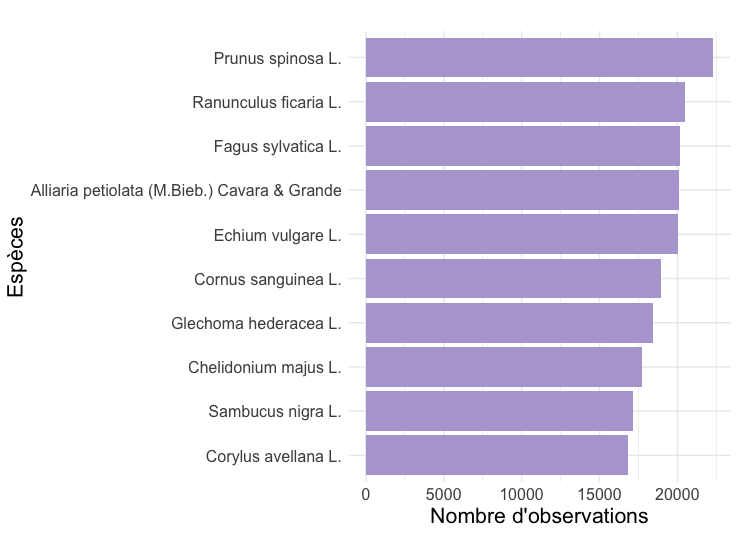
\includegraphics[scale=0.3]{images/10_Most_Observed_Species.png}
  \caption{Histogramme des $10$ espèces végétales les plus osbervées}
  \label{fig1}
\end{figure}

Comme le montre la figure $1$, les espèces les plus fréquemment photographiées par les utilisateurs de Pl@ntnet sont essentiellement des arbres vivaces, certains fruitiers, ou des fleurs comestibles, aux propriétés curatives et qui peuvent être aperçues dans toute la zone géographique étudiée. Le \textit{Prunus Spinosa L.} ou, plus communément, prunellier, arrive en tête des observations, suivi par d'autres espèces communes comme le \textit{Fagus Sylvatica L.} (hêtre commun) ou encore le \textit{Corylus avellana L.} (noisetier commun).

\vspace{0.2cm}

Cette distribution n'est pas surprenante puisqu'elle reflète à la fois l'abondance de ces espèces dans l'écosystème méditerranéen et l'intérêt qu'elle suscite auprès du grand public, soit pour leur valeur décorative, soit pour leurs usages alimentaires ou médicinaux.

\vspace{0.2cm}

À l'autre extrémité, les espèces les moins observées (avec parfois une seule occurrence dans la base) correspondent généralement à des plantes rares, présentes dans des zones très restreintes, ou simplement moins reconnaissables par le grand public.

\subsubsection{Relation entre fréquence d'observation et probabilités}

Au-delà de la simple fréquence d'apparition des espèces, qui semble seulement impliquer un intérêt de l'observateur, nous nous sommes intéressées à la relation entre cette fréquence et la qualité des prédictions de l'algorithme d'intelligence artificielle. Pour cela, nous avons analysé les scores "Top $1$" attribués par le système, c'est-à-dire la probabilité associée à l'espèce la plus probable selon l'algorithme. Nous avons obtenu les graphiques suivants :

\begin{figure}[H]
\centering
\begin{minipage}{0.5\textwidth}
  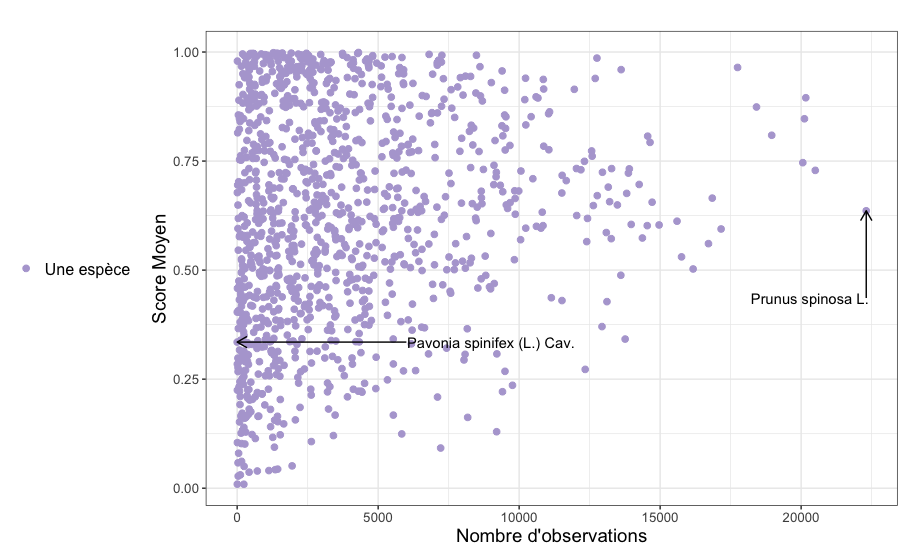
\includegraphics[width=0.8\linewidth]{images/mean_rd.png}
\end{minipage}%
\begin{minipage}{0.5\textwidth}
  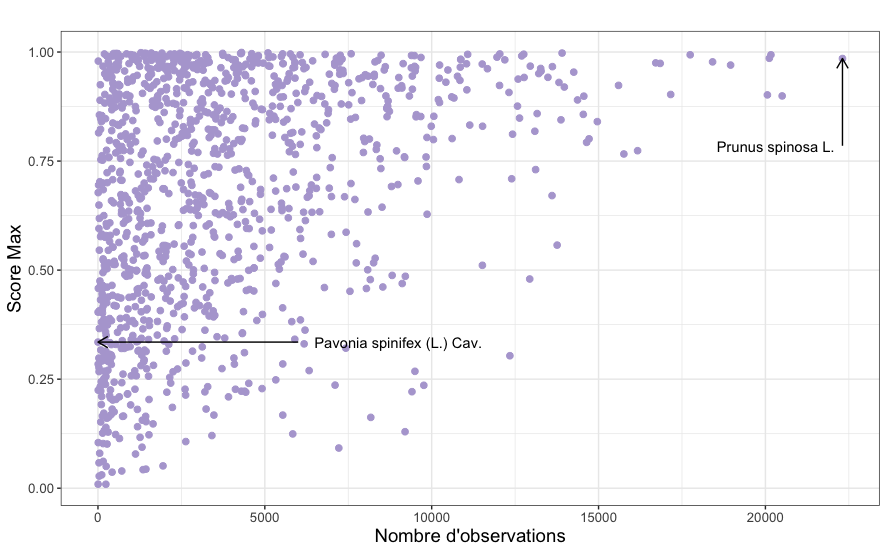
\includegraphics[width=0.8\linewidth]{images/max_rd.png}
\end{minipage}
\caption{Nuages de points de la moyenne des scores ou des scores max en fonction du nombre d'observations}
\end{figure}

Ces deux graphiques révèlent plusieurs phénomènes intéressants.

Contrairement à ce que l'on pourrait intuitivement penser, il n'existe pas de relation linéaire évidente entre la fréquence d'observation d'une espèce et la confiance moyenne du système dans ses prédictions. Des espèces très fréquentes peuvent recevoir des scores moyens relativement bas, tandis que certaines espèces rares obtiennent des scores élevés.

\vspace{0.2cm}

Le \textit{Prunus Spinosa L.}
, l'espèce la plus observée, présente un score moyen relativement élevé (proche de $0,6$), ce qui suggère que le système est généralement confiant dans son identification. Cela peut s'expliquer par ses caractéristiques morphologiques distinctives et possiblement par la qualité généralement bonne des photos de cette espèce commune.

\vspace{0.2cm}

Certaines espèces n'ayant qu'une seule observation présentent des scores très élevés, proches de $1$. Ce phénomène pourrait s'expliquer par le processus d'apprentissage du modèle : si l'intelligence artificielle a été entraînée sur des images similaires à cette unique observation dans notre jeu de données, elle peut la reconnaître avec une grande confiance.

\subsubsection{Facteurs influençant la qualité des prédictions}

Plusieurs facteurs peuvent expliquer la variabilité observée dans les scores de prédiction : 
\begin{itemize}
    \item \textbf{Qualité des images :} les photos floues, mal cadrées, prises de trop loin ou dans des conditions d'éclairage défavorables réduisent considérablement la performance de l'algorithme.
    \item \textbf{Confusion entre espèces similaires :} certaines espèces appartenant au même genre partagent des caractéristiques morphologiques très proches, ce qui peut induire l'algorithme en erreur. Par exemple, différentes espèces de chênes ou de roses peuvent être difficiles à distinguer même pour des botanistes expérimentés.
    \item \textbf{Stade de développement de la plante :} une même espèce peut présenter des aspects très différents selon la saison (avec ou sans feuilles, en fleur ou non, avec ou sans fruit, etc.), ce qui peut affecter la confiance du système dans ses prédictions.
    \item \textbf{Organe photographié :} les fleurs sont généralement plus distinctives et permettent une identification plus fiable que les feuilles ou les tiges, qui peuvent présenter plus de similarités entre espèces.
    \item \textbf{Effet d'apprentissage sur des images spécifiques :} comme mentionné précédemment, certaines espèces rares peuvent obtenir des scores très élevés si l'image soumise est similaire à celle utilisée pour l'entraînement du modèle.
\end{itemize}

\subsubsection{Impact du choix de l'utilisateur}

Les espèces associées aux probabilités Top 1 ne sont pas systématiquement celles choisies par l'observateur, qui peut décider de désigner une espèce de probabilités plus faibles également proposées par l'IA ou opter pour une tout autre espèce. Des utilisateurs n'ayant pas observé eux-mêmes, sur place, peuvent également choisir une espèce à l'instar de l'observateur. Nous avons admis par vote majoritaire que l'observateur a plus de poids que les autres votants, sauf si les votants externes sont plus nombreux à valider une réponse qui diffère de l'observateur. Observons sur un échantillon plus restreint du jeu de données les différences entre le Top 1 et le vote majoritaire. 
\begin{figure}[H]
    \centering
    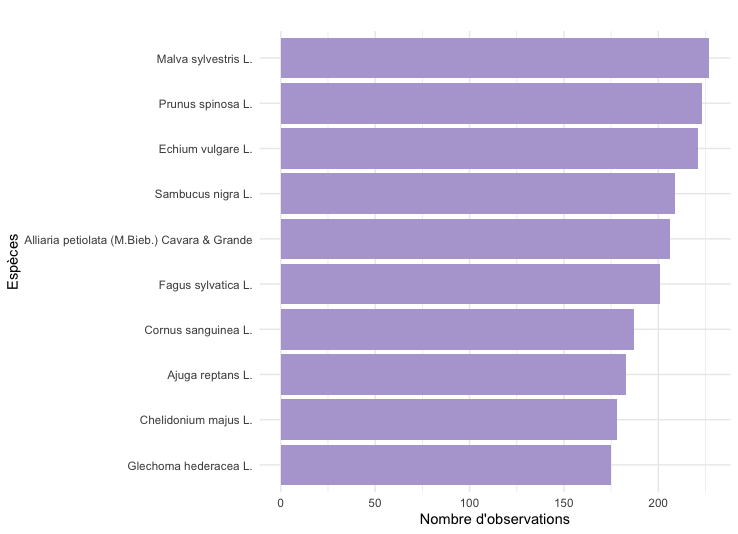
\includegraphics[scale=0.3]{images/10_Most_Observed_Species_Users.png}
    \caption{Histogramme des $10$ espèces végétales les plus osbervées}
    \label{fig2}
\end{figure}67461

Si \textit{Prunus Spinosa L.} est toujours présente dans ce graphique, c'est l'espèce \textit{Malva sylvestris L.}, une fleur au mauve intense, qui est en tête. Sur ces $67 461$ observations (un centième des données totales), elle est donc la plus souvent choisie par les utilisateurs. Ce graphique seul indique que l'espèce prédite en première par l'IA, celle en qui l'algorithme est le plus confiant, n'est pas toujours ce que l'utilisateur compte choisir. Il est envisageable que les espèces proposées par l'IA dans son Top K se ressemblent : il existe par exemple plusieurs espèces d'iris ou de lotus partageant donc des caractéristiques communes, on parle de "familles".
\begin{figure}[H]
    \centering
    \begin{minipage}{0.5\textwidth}
      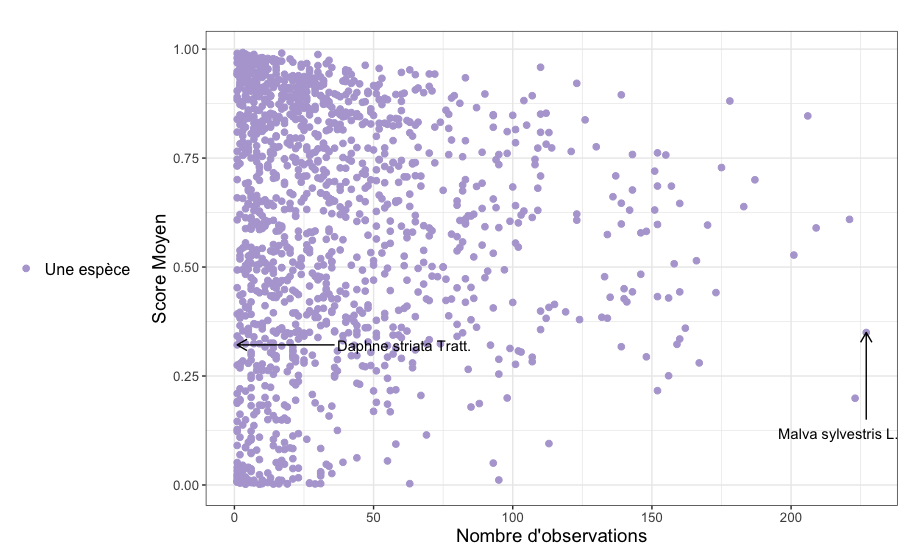
\includegraphics[width=0.8\linewidth]{images/mean_rd_users.png}
    \end{minipage}%
    \begin{minipage}{0.5\textwidth}
      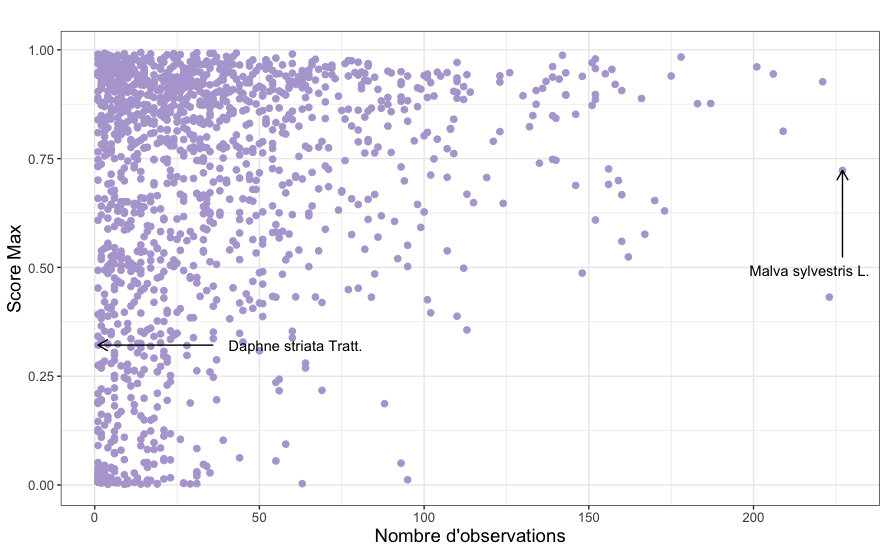
\includegraphics[width=0.8\linewidth]{images/max_rd_users.png}
    \end{minipage}
    \caption{Nuages de points de la moyenne des scores ou des scores max en fonction du nombre d'observations}
\end{figure}

La plante n'ayant été choisie qu'une seule fois dans cet échantillon est \textit{Daphne striata Tratt.}, un arbrisseau à fines fleurs roses et fruits rouges. Son score est pourtant assez bas, nous pouvons imaginer qu'elle n'était proposée par l'application qu'en deuxième ou troisième position. Pour ce qui est de la Mauve, sa probabilité est élevée, elle est possiblement le Top 1 de l'algorithme, ce qui entraîne le choix de l'observateur. Outre ces deux espèces, nous remarquons qu'il y a plusieurs espèces aux scores très proches de $0$ qui ont été choisies, soit parce que l'IA n'était pas confiante et a proposé de nombreuses options ayant des probabilités minimes, soit parce que les votants ont eux-mêmes été chercher une espèce en particulier parmi les espèces les moins évidentes selon l'IA.

\vspace{0.2cm}

Ces observations préliminaires nous ont confirmé la nécessité d'une approche adaptative pour la présentation des résultats aux utilisateurs. En effet, un système qui proposerait un nombre fixe d'espèces candidates serait soit trop restrictif dans les cas difficiles (risquant d'oublier la bonne espèce), soit trop verbeux dans les cas simples (noyant l'utilisateur sous des propositions inutiles).

\vspace{0.2cm}

La prédiction conforme, que nous allons introduire dans la section suivante, offre plus précisément le cadre mathématique nécessaire pour adapter dynamiquement le nombre de suggestions en fonction de la difficulté de chaque cas d'identification.

%%%%%%%%%%%%%%%%%%%%%%%%%%%%%%%%%%%%%%%%%%%%%%%%%%%%%%%%%%%%%%%%%%%%%%%%%%%%%%%%

\subsection{Prédiction conforme}

La prédiction conforme est un cadre statistique qui permet de quantifier l'incertitude des prédictions faites par des algorithmes d'apprentissage automatique, y compris les réseaux de neurones utilisés dans Pl@ntnet. Contrairement aux autres approches comme le bootstrap qui reposent sur des hypothèses paramétriques, la prédiction conforme offre des garanties de couverture valables même pour des échantillons de taille finie, sans hypothèses fortes sur la distribution des données (\cite{ShaferVovk}).

\subsubsection{Cadre mathématiques}

Nous considérons $(X_i, Y_i)$ des paires constituées de caractéristiques ($X_i$) et de réponses ($Y_i$) indépendantes et identiquement distribuées issues d'une distribution inconnue $P$, avec $i = 1, \dots, n$. Dans notre contexte, $X_i$ représente les caractéristiques extraites d'une image de plante, et $Y_i \in \{1, 2, \dots, K\}$ l'indice de la véritable espèce parmi les $K$ possibles. Notre espace des caractéristiques est $X = \mathbb R^d$ et notre espace des réponses est $Y = \mathbb R$.

\vspace{0.2cm}

L'objectif de la prédiction conforme est de construire, pour un nouvel échantillon $X_{n+1}$, un ensemble de prédiction $\hat{C}_n(X_{n+1}) \subseteq \{1, 2, \dots, K\}$ qui contienne la vraie classe $Y_{n+1}$ avec une probabilité d'au moins $1 - \alpha$, où $\alpha \in ]0,1[$ est un niveau d'erreur fixé à l'avance : 
$$ \mathbb P(Y_{n+1} \in \hat C_n (X_{n+1}) \geq 1 - \alpha) $$

\vspace{0.2cm}

Cette garantie de couverture est valable sous l'hypothèse que les paires $(X_i, Y_i)$ soient échangeables, une condition plus faible que l'indépendance et l'identité de distribution.

\vspace{0.2cm}

De plus, cela nécessite certaines conditions supplémentaires. La première va être de ne pas poser d'hypothèse sur $P$. Ensuite, nous ne devons pas non plus utiliser toutes les prédictions possibles, car nous voulons un nombre de prédictions fini, mais également raisonnable. Pour finir, nous voulons adapter notre stratégie à la dureté du problème, c'est-à-dire que plus il est facile de prédire $Y_{n+1}$ à partir de $X_{n+1}$ et plus notre ensemble $\hat C_n(X_{n+1})$ devra être petit.

\vspace{0.2cm}

Cela est tout à fait possible avec une distribution infinie dans des conditions standard (convergence du quantile de l'échantillon vers le quantile de la population). Mais, étant donné que nous sommes dans des conditions réelles, nous nous intéressons ici à des échantillons finis.

\subsubsection{Construction des ensembles de prédiction}

La construction des ensembles de prédiction conforme repose sur l'utilisation d'une fonction de score $s : \mathcal{X} \times \mathcal{Y} \rightarrow \mathbb{R}$ qui mesure la non-conformité (ou taux d'erreur) d'une paire (observation, classe). Plus cette valeur est élevée et moins l'observation et la classe sont conformes aux données d'entraînement.

\vspace{0.2cm}

La procédure de base comporte trois étapes : 
\begin{itemize}
    \item \textbf{Définition des vraies étiquettes :} pour les observations expertes, nous sommes partis du principe que, quand un expert avait donné une étiquette, elle était considérée comme correcte. Pour les observations non expertes, nous avons appliqué la méthode du vote majoritaire, que nous détaillerons par la suite, pour déterminer quel était le vrai label.
    \item \textbf{Calcul des scores de non-conformité :} pour chaque paire $(X_i, Y_i)$, on calcule un score $s(X_i, Y_i)$ qui indique à quel point cette paire est inhabituelle selon le modèle.
    \item \textbf{Construction de l'ensemble de prédiction :} pour un nouvel exemple $X_{n+1}$, on construit l'ensemble de prédiction en incluant toutes les classes $y$ pour lesquelles le score $s(X_{n+1}, y)$ est inférieur au quantile $(1- \alpha)$.
\end{itemize}

Cette procédure garantit que la probabilité que l'ensemble de prédiction contienne la vraie classe est d'au moins $1- \alpha$, c'est-à-dire $95\%$.

\subsubsection{Fonctions de scores}

Dans notre contexte de classification, plusieurs fonctions de score sont possibles. Nous avons donc choisi d'explorer deux principaux scores que sont la prédiction de la vraie classe et le score cumulatif.

\vspace{0.2cm}

Le score basé sur la probabilité de la vraie classe (\cite{Vovk}) se calcule comme suit : 
$$ s_1(X_i, Y_i) = 1 - p_{Y_i}(X_i) $$ où $p_{Y_i}(X_i)$ est la probabilité prédite par le modèle pour le vrai label. Plus cette probabilité est élevée et plus le score est faible, ce qui est souhaitable.

\vspace{0.2cm}

Le score cumulatif APS (Adaptive Prediction Sets) se calcule comme suit : 
$$ s_2(X_i, Y_i) = \sum_{j=1}^{r(X_i, Y_i)-1} p_{(j)}(X_i) $$ où $p_{(j)}(X_i)$ représente la $j$-ième plus grande probabilité prédite par le modèle pour l'observation $X_i$, et $r(X_i, Y_i)$ est le rang de la vraie classe $Y_i$ dans ce classement. Cette fonction de score, introduite par \cite{Romano}, permet de construire des ensembles de prédiction dont la taille s'adapte à la difficulté du problème.

\vspace{0.2cm}

Le score $s_2$ présente l'avantage de produire des ensembles de prédiction dont la taille varie en fonction de la confiance du modèle : pour les cas faciles où la vraie classe reçoit une probabilité dans celles les plus élevées (donc un rang faible), la somme sera petite et l'ensemble de prédiction contiendra peu de classes. Au contraire, pour les cas difficiles, l'ensemble sera plus grand pour maintenir la garantie de couverture.

\subsubsection{Spécificités de notre approche}

Dans le contexte de notre projet sur Pl@ntent, nous avons dû adapter la méthode standard pour tenir compte de plusieurs spécificités.

\vspace{0.2cm}

Comme indiqué plus tôt, les scores que nous avons récupérés étaient tronqués, ne conservant que les probabilités supérieures à un certain seuil ($1/1000$). Pour gérer ce problème, nous avons décidé de considérer que les classes non présentes dans la liste avaient une probabilité de $1/1000$, ce qui nous a permis d'appliquer les formules de scores sans souci.

\vspace{0.2cm}

Une étape importante consistait à établir une vérité terrain fiable pour chaque observation, c'est-à-dire à déterminer quel label était le vrai pour chaque observation. Pour les observations avec le vote d'un utilisateur expert, nous avons directement utilisé leur identification comme référence absolue. Pour les observations sans validation experte, nous avons appliqué une méthode de vote majoritaire parmi les identifications fournies par les utilisateurs. C'est-à-dire que nous avons compté le nombre de réponses par label donné, en donnant un poids plus important à l'utilisateur ayant pris la photo, car c'est le seul à avoir réellement vu la plante, et avons posé que c'était l'espèce avec le plus de votes qui était le label correct. En cas d'égalité entre deux espèces candidates, nous avons sélectionné aléatoirement l'une d'entre elles.

\vspace{0.2cm}

Ces adaptations nous ont permis d'appliquer avec succès le cadre de prédiction conforme à notre problématique d'identification des plantes, pour pouvoir par la suite déterminer nos ensembles de prédiction.

%%%%%%%%%%%%%%%%%%%%%%%%%%%%%%%%%%%%%%%%%%%%%%%%%%%%%%%%%%%%%%%%%%%%%%%%%%%%%%%%

\subsection{Méthodologie d'évaluation et validation croisée}

Au-delà de la définition théorique des scores de non-conformité, nous avons dû concevoir une méthodologie pour évaluer l'efficacité de notre approche conforme. Pour garantir des résultats statistiquement valides, nous avons adopté une stratégie de division des données qui permet à la fois de calibrer nos modèles, mais également d'en tester les performances sur des échantillons indépendants pour pouvoir les comparer.

\subsubsection{Division des données}

Notre stratégie de division s'articule autour de deux critères principaux : l'expertise des utilisateurs et le type de score utilisé. Cette approche nous a conduit à créer quatre configurations distinctes : 
\begin{itemize}
    \item \textbf{Modèle $1$ :} score $s_1$ (probabilité de la vraie classe) avec calibration sur toutes les données non-expertes et test sur la moitié des données expertes.
    \item \textbf{Modèle $2$ :} score $s_1$ avec calibration sur la moitié des données expertes et test sur l'autre moitié des données expertes.
    \item \textbf{Modèle $3$ :} score $s_2$ (score cumulatif APS) avec calibration sur toutes les données non-expertes et test sur la moitié des données expertes.
    \item \textbf{Modèle $4$ :} score $s_2$ avec calibration sur la moitié des données expertes et test sur l'autre moitié des données expertes.
\end{itemize}

\vspace{0.2cm}

Nous avons représenté cette configuration comme suit : 
\begin{figure}[H]
    \centering
    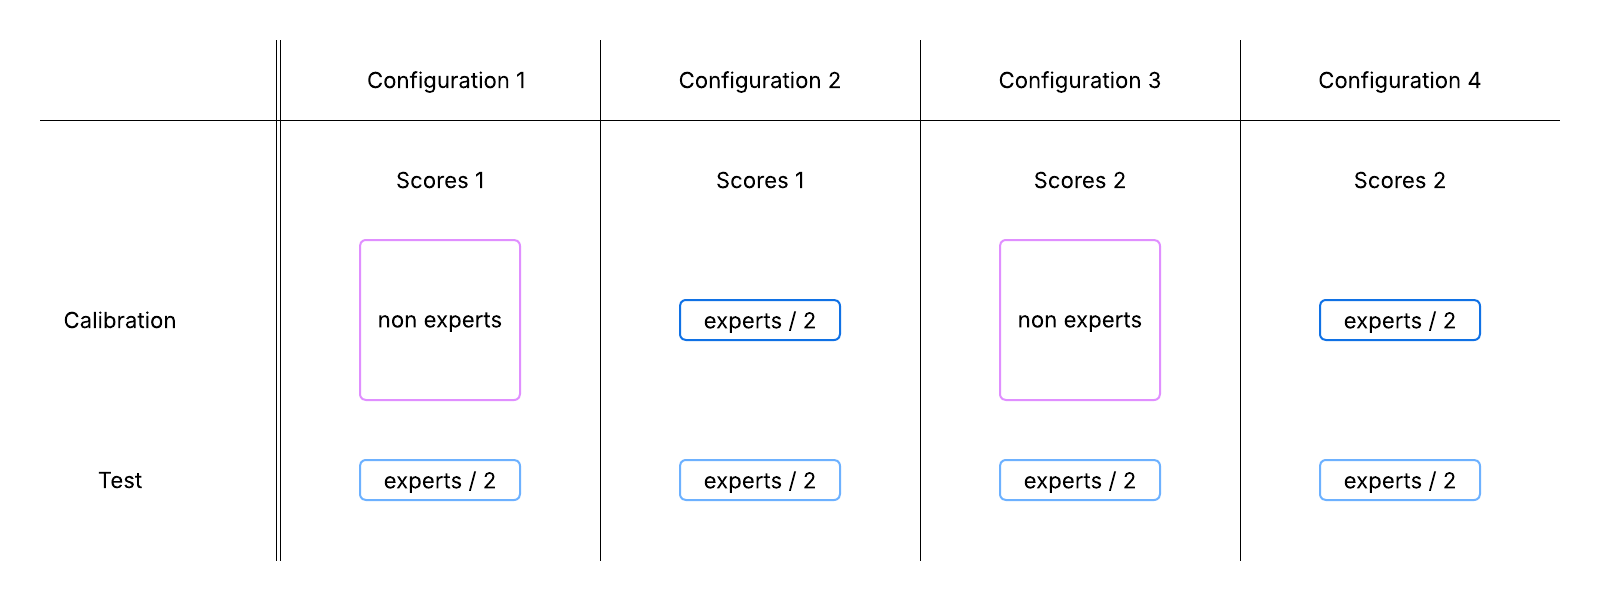
\includegraphics[scale=0.6]{images/Models.png}
    \caption{Représentation des modèles}
    \label{models}
  \end{figure}

\vspace{0.2cm}

Cette structure nous permet d'évaluer non seulement l'impact du choix de la fonction de score ($s_1$ ou $s_2$), mais également l'influence de la qualité des données de calibration (expertes avec peu de données ou non expertes avec beaucoup de données) sur les performances finales.

\vspace{0.2cm}

Pour assurer la représentativité de nos échantillons, nous avons divisé les données expertes aléatoirement et avons vérifié que les deux groupes créés étaient bien similaires en termes de scores.

\subsubsection{Calcul des quantiles}

Une fois les données divisées, l'étape suivante a consisté à calculer les quantiles des scores de non-conformité qui nous permettraient de construire nos ensembles de prédiction avec le niveau de garantie souhaitée de $95\%$.

\vspace{0.2cm}

Pour chaque configuration, nous avons commencé par récupérer les scores pour chaque observation du jeu de calibration que nous avons précédemment calculé. Puis, nous avons calculé le quantile $\frac{[(n+1)(1 - \alpha)]}{n}$, où $\alpha = 0,05$ représente notre niveau d'erreur souhaité et $n$ est le nombre d'observations dans notre ensemble d'apprentissage. Enfin, nous avons implémenté une fonction qui, pour toute nouvelle observation, calcule les scores de non-conformité pour chaque classe possible et inclut dans l'ensemble de prédiction toutes les classes dont le score est inférieur au quantile calculé précédemment.

\vspace{0.2cm}

Pour le calcul concret du quantile, nous avons utilisé la fonction quantile de Python, adaptée pour notre large volume de données. Nous avons obtenu les résultats suivants : 

\begin{center}
    \begin{tabular}{|l|c|}
        \hline
        Configuration & Quantile calculé \\
        \hline
        Score $s_1$ + données non expertes & $0.9990$ \\
        Score $s_1$ + données expertes & $0.9649$ \\
        Score $s_2$ + données non expertes & $0.7618$ \\
        Score $s_2$ + données expertes & $0.5614$ \\
        \hline
        \end{tabular}
    \end{center}

\vspace{0.2cm}

Ces quantiles sont des seuils critiques : un score élevé indique une faible confiance, donc, pour le $s_1$, nous incluons toutes les classes dont le score est inférieur au quantile. Pour le $s_2$, nous incluons les classes jusqu'à ce que leur somme cumulée dépasse le quantile.

\vspace{0.2cm}

Analysons le tableau : 

\begin{itemize}
    \item Score s1 (non experts) de $0.9990$ : un seuil très élevé, ce qui signifie que la plupart des données non expertes ont des valeurs faibles, à l'exception d'une petite portion qui dépasse ce seuil.
    \item Score s1 (experts) de $0.9649$ : un seuil plus bas que les non-experts, ce qui indique que les données des experts sont plus cohérentes et ont une répartition moins extrême.
    \item Score s2 (non experts) de $0.7618$ : comparé à s1, ce seuil est plus bas, ce qui montre que la variabilité de ce score est moins marquée dans les données des non-experts.
    \item Score s2 (experts) de $0,5614$ : le plus bas des quatre seuils, ce qui pourrait signifier que les scores s2 des experts sont généralement plus homogènes et moins extrêmes.
\end{itemize}

\subsubsection{Calcul des autres variables}

Pour évaluer l'efficacité de notre approche de prédiction conforme, nous avons mesuré deux métriques principales sur nos ensembles de test que sont le taux de couverture et leur taille moyenne. 

\vspace{0.2cm}

Le taux de couverture représente la proportion des observations pour lesquelles la vraie classe est incluse dans l'ensemble de prédiction. Idéalement, ce taux devrait être supérieur ou égal à $1- \alpha$, c'est-à-dire à $95\%$.

\vspace{0.2cm}

De plus, nous avons calculé la taille moyenne des ensembles de prédiction, qui correspond au nombre moyen de classes incluses dans les ensembles de prédiction. Pour une meilleure expérience utilisateur, cette taille doit être aussi petite que possible tout en maintenant le taux de couverture cible.

\vspace{0.2cm}

Les résultats que nous avons obtenus seront détaillés dans la partie suivante, afin de pouvoir comparer nos modèles en même temps.

\section{Résultats et discussion}

Après avoir défini notre méthodologie et implémenté les algorithmes correspondants, nous avons procédé à l'évaluation systématique des quatre configurations décrites précédemment à l'aide des variables calculées. Cette section présente les résultats obtenus, analyse leurs implications en pratique et discute de la généralisation de notre approche à l'ensemble des données Pl@ntnet.

\subsection{Analyse comparative}

À la suite de nos calculs pour mesurer l'efficacité de nos modèles, les résultats obtenus pour nos quatre configurations sont résumés dans le tableau suivant :

\begin{center}
\begin{tabular}{|c|c|c|c|}
    \hline
    Configuration & Taux de couverture & Taille moyenne & Taille médiane \\
    \hline
    $s_1$ + non expert & $100\%$ & $??$ & $??$ \\
    $s_1$ + expert & $94.82\%$ & $??$ & $??$ \\
    $s_2$ + non expert & $97.98\%$ & $0.06$ & $??$ \\
    $s_2$ + expert & $94.91\%$ & $0.06$ & $??$ \\
    \hline
    \end{tabular}
\end{center}
    
Ces résultats révèlent plusieurs tendances importantes ????

\subsection{Traitement du jeu de données complet}

Encouragés par les résultats prometteurs obtenus sur notre échantillon de $\num{67 466}$ observations, nous avons entrepris d'étendre notre approche à l'intégralité des $\num{6 699 593}$ observations de la base de données Pl@ntnet-CrowdSWE. Cette mise à l'échelle présentait des défis considérables, principalement sur le plan technique.

\vspace{0.2cm}

Le traitement de près de $7$ millions d'observations, chacune associée à un vecteur de probabilités potentiellement long (jusqu'à plusieurs centaines de classes candidates), a nécessité plusieurs adaptations. Mais malgré des optimisations, le traitement complet des données a nécessité plusieurs jours de calcul sur des machines puissantes, soulignant la difficulté que représente l'application de méthodes de prédiction conforme à des jeux de données massifs.

\vspace{0.2cm}

Les analyses sur l'ensemble complet des données étaient encore en cours au moment de la rédaction de ce rapport, mais les résultats préliminaires obtenus ont pu tout de même être traités et donner de la matière à ce rapport.

\subsection{Perspectives d'intégration dans l'application}

L'intégration de notre système de prédiction conforme dans l'application Pl@ntnet nécessiterait quelques ajustements supplémentaires :
\begin{itemize}
    \item \textbf{Calcul en temps réel} : notre approche actuelle, basée sur des calculs de quantiles préalables, pourrait être adaptée pour permettre un calcul en temps réel des ensembles de prédiction pour chaque nouvelle observation soumise par un utilisateur.
    \item \textbf{Mise à jour périodique} : les quantiles utilisés pour déterminer les seuils de décision devraient être recalculés périodiquement (par exemple, mensuellement) pour refléter l'évolution du modèle de base et des distributions de probabilités qu'il génère.
    \item \textbf{Interface utilisateur} : la présentation des résultats pourrait être adaptée pour expliquer clairement aux utilisateurs la nature adaptative des suggestions et la garantie statistique associée.
\end{itemize}

\vspace{0.2cm}

Si le temps l'avait permis, nous aurions souhaité développer un exemple d'interface utilisateur intégrant notre système de prédiction conforme, afin de démontrer concrètement l'amélioration potentielle de l'expérience utilisateur.

%%%%%%%%%%%%%%%%%%%%%%%%%%%%%%%%%%%%%%%%%%%%%%%%%%%%%%%%%%%%%%%%%%%%%%%%%%%%%%%%
%%%%%%%%%%%%%%%%%%%%%%%%%%%%%%%%%%%%%%%%%%%%%%%%%%%%%%%%%%%%%%%%%%%%%%%%%%%%%%%%

\section{Conclusion}

Dans ce projet, nous avons abordé la problématique de l'incertitude dans l'identification automatique des plantes, un défi majeur pour l'application Pl@ntnet qui repose sur des données collectées par une vaste communauté d'utilisateurs aux expertises avérées. Notre approche s'est articulée autour de la prédiction conforme, un cadre statistique qui permet de transformer des sorties probabilistes d'un modèle de classification en ensembles de prédiction dotés de garanties de couverture.

\vspace{0.2cm}

À partir d'un jeu de données de plus de $6$ millions d'observations d'espèces végétales en Europe du Sud-Ouest, nous avons développé une méthodologie permettant d'adapter dynamiquement le nombre de suggestions d'espèces en fonction de la difficulté d'identification de chaque image. 

\vspace{0.2cm}

Cette approche présente plusieurs avantages par rapport au système actuel de Pl@ntnet, notamment parce qu'elle fournit une garantie statistique que la vraie espèce est incluse dans l'ensemble des suggestions avec une probabilité d'au moin $95\%$. De plus, elle réduit le nombre de suggestions dans les cas faciles, tout en élargissant les propositions dans les cas ambigus pour maintenir la garantie de couverture.

\vspace{0.2cm}

Nos expériences ont démontré la supériorité du score ?? par rapport à ??, ainsi que l'importance de la qualité des données de calibration. La configuration combinant le score ?? avec une calibration sur données ?? a produit les résultats les plus convaincants, avec une taille moyenne d'ensemble de prédiction de ??, tout en maintenant le taux de couverture au-dessus de $95\%$.

\vspace{0.2cm}

Bien que le traitement de l'intégralité des $7$ millions d'observations ait posé des défis techniques nécessitant plusieurs jours de calcul, les résultats préliminaires sur notre échantillon démontrent la faisabilité de nos modèles.

\vspace{0.2cm}

Ce projet ouvre plusieurs perspectives intéressantes pour des travaux futurs :

\begin{itemize}
    \item L'exploration d'autres fonctions de score potentiellement plus performantes.
    \item L'adaptation de notre approche pour prendre en compte d'autres types d'incertitude, comme l'incertitude liée à la qualité des images ou à la variabilité saisonnière des caractéristiques morphologiques.
\end{itemize}

\vspace{0.2cm}

En conclusion, notre étude démontre le potentiel de la prédiction conforme pour améliorer la fiabilité et l'expérience utilisateur des systèmes d'identification automatique des plantes, et plus généralement, de tout système de classification automatique confronté à des données de qualité variable et à des situations d'ambiguïté naturelle.

\printbibliography

\end{document}

